\documentclass[twoside]{book}

% Packages required by doxygen
\usepackage{fixltx2e}
\usepackage{calc}
\usepackage{doxygen}
\usepackage[export]{adjustbox} % also loads graphicx
\usepackage{graphicx}
\usepackage[utf8]{inputenc}
\usepackage{makeidx}
\usepackage{multicol}
\usepackage{multirow}
\PassOptionsToPackage{warn}{textcomp}
\usepackage{textcomp}
\usepackage[nointegrals]{wasysym}
\usepackage[table]{xcolor}

% Font selection
\usepackage[T1]{fontenc}
\usepackage[scaled=.90]{helvet}
\usepackage{courier}
\usepackage{amssymb}
\usepackage{sectsty}
\renewcommand{\familydefault}{\sfdefault}
\allsectionsfont{%
  \fontseries{bc}\selectfont%
  \color{darkgray}%
}
\renewcommand{\DoxyLabelFont}{%
  \fontseries{bc}\selectfont%
  \color{darkgray}%
}
\newcommand{\+}{\discretionary{\mbox{\scriptsize$\hookleftarrow$}}{}{}}

% Page & text layout
\usepackage{geometry}
\geometry{%
  a4paper,%
  top=2.5cm,%
  bottom=2.5cm,%
  left=2.5cm,%
  right=2.5cm%
}
\tolerance=750
\hfuzz=15pt
\hbadness=750
\setlength{\emergencystretch}{15pt}
\setlength{\parindent}{0cm}
\setlength{\parskip}{3ex plus 2ex minus 2ex}
\makeatletter
\renewcommand{\paragraph}{%
  \@startsection{paragraph}{4}{0ex}{-1.0ex}{1.0ex}{%
    \normalfont\normalsize\bfseries\SS@parafont%
  }%
}
\renewcommand{\subparagraph}{%
  \@startsection{subparagraph}{5}{0ex}{-1.0ex}{1.0ex}{%
    \normalfont\normalsize\bfseries\SS@subparafont%
  }%
}
\makeatother

% Headers & footers
\usepackage{fancyhdr}
\pagestyle{fancyplain}
\fancyhead[LE]{\fancyplain{}{\bfseries\thepage}}
\fancyhead[CE]{\fancyplain{}{}}
\fancyhead[RE]{\fancyplain{}{\bfseries\leftmark}}
\fancyhead[LO]{\fancyplain{}{\bfseries\rightmark}}
\fancyhead[CO]{\fancyplain{}{}}
\fancyhead[RO]{\fancyplain{}{\bfseries\thepage}}
\fancyfoot[LE]{\fancyplain{}{}}
\fancyfoot[CE]{\fancyplain{}{}}
\fancyfoot[RE]{\fancyplain{}{\bfseries\scriptsize Generated by Doxygen }}
\fancyfoot[LO]{\fancyplain{}{\bfseries\scriptsize Generated by Doxygen }}
\fancyfoot[CO]{\fancyplain{}{}}
\fancyfoot[RO]{\fancyplain{}{}}
\renewcommand{\footrulewidth}{0.4pt}
\renewcommand{\chaptermark}[1]{%
  \markboth{#1}{}%
}
\renewcommand{\sectionmark}[1]{%
  \markright{\thesection\ #1}%
}

% Indices & bibliography
\usepackage{natbib}
\usepackage[titles]{tocloft}
\setcounter{tocdepth}{3}
\setcounter{secnumdepth}{5}
\makeindex

% Hyperlinks (required, but should be loaded last)
\usepackage{ifpdf}
\ifpdf
  \usepackage[pdftex,pagebackref=true]{hyperref}
\else
  \usepackage[ps2pdf,pagebackref=true]{hyperref}
\fi
\hypersetup{%
  colorlinks=true,%
  linkcolor=blue,%
  citecolor=blue,%
  unicode%
}

% Custom commands
\newcommand{\clearemptydoublepage}{%
  \newpage{\pagestyle{empty}\cleardoublepage}%
}

\usepackage{caption}
\captionsetup{labelsep=space,justification=centering,font={bf},singlelinecheck=off,skip=4pt,position=top}

%===== C O N T E N T S =====

\begin{document}

% Titlepage & ToC
\hypersetup{pageanchor=false,
             bookmarksnumbered=true,
             pdfencoding=unicode
            }
\pagenumbering{alph}
\begin{titlepage}
\vspace*{7cm}
\begin{center}%
{\Large My Project }\\
\vspace*{1cm}
{\large Generated by Doxygen 1.8.13}\\
\end{center}
\end{titlepage}
\clearemptydoublepage
\pagenumbering{roman}
\tableofcontents
\clearemptydoublepage
\pagenumbering{arabic}
\hypersetup{pageanchor=true}

%--- Begin generated contents ---
\chapter{Namespace Index}
\section{Namespace List}
Here is a list of all namespaces with brief descriptions\+:\begin{DoxyCompactList}
\item\contentsline{section}{\hyperlink{namespacevis}{vis} }{\pageref{namespacevis}}{}
\end{DoxyCompactList}

\chapter{Class Index}
\section{Class List}
Here are the classes, structs, unions and interfaces with brief descriptions\+:\begin{DoxyCompactList}
\item\contentsline{section}{\hyperlink{classDataset}{Dataset} \\*A class for the dataset  A constructor to initialize with number of points and an array to store points }{\pageref{classDataset}}{}
\item\contentsline{section}{\hyperlink{classerrorxy}{errorxy} \\*A class for error  The slope,intercept and error values }{\pageref{classerrorxy}}{}
\item\contentsline{section}{\hyperlink{classpoint}{point} \\*A class for point  The coordinates and a constructor }{\pageref{classpoint}}{}
\end{DoxyCompactList}

\chapter{File Index}
\section{File List}
Here is a list of all files with brief descriptions\+:\begin{DoxyCompactList}
\item\contentsline{section}{\hyperlink{bestfit_8cpp}{bestfit.\+cpp} \\*Basic functionality.  This file has all the classes and functions needed to find the bestfit line. It is called by the Python script everytime the slider is changed }{\pageref{bestfit_8cpp}}{}
\item\contentsline{section}{\hyperlink{vis_8py}{vis.\+py} }{\pageref{vis_8py}}{}
\end{DoxyCompactList}

\chapter{Namespace Documentation}
\hypertarget{namespacevis}{}\section{vis Namespace Reference}
\label{namespacevis}\index{vis@{vis}}
\subsection*{Functions}
\begin{DoxyCompactItemize}
\item 
def \hyperlink{namespacevis_a987b76332d0d03b66af97331e5e4b442}{get\+Val} (event)
\end{DoxyCompactItemize}
\subsection*{Variables}
\begin{DoxyCompactItemize}
\item 
int \hyperlink{namespacevis_a670f391917319e53a1373004ad47a325}{n\+\_\+points} = 10
\item 
\hyperlink{namespacevis_a4086117aa0dbd872a99b2f3738d56ae6}{x\+\_\+pure} = np.\+linspace(-\/\hyperlink{namespacevis_a670f391917319e53a1373004ad47a325}{n\+\_\+points},\hyperlink{namespacevis_a670f391917319e53a1373004ad47a325}{n\+\_\+points},\hyperlink{namespacevis_a670f391917319e53a1373004ad47a325}{n\+\_\+points})
\item 
\hyperlink{namespacevis_ac14aca4ab4de023eb6759df589da3396}{y\+\_\+pure} = \hyperlink{namespacevis_a4086117aa0dbd872a99b2f3738d56ae6}{x\+\_\+pure}
\item 
list \hyperlink{namespacevis_ac930396acd65d715184cfd4ae2df301c}{noise\+\_\+points} = \mbox{[}i\mbox{[}0\mbox{]} for i in (\hyperlink{namespacevis_a670f391917319e53a1373004ad47a325}{n\+\_\+points}$\ast$np.\+random.\+rand(\hyperlink{namespacevis_a670f391917319e53a1373004ad47a325}{n\+\_\+points},1) -\/ \hyperlink{namespacevis_a670f391917319e53a1373004ad47a325}{n\+\_\+points}/2)\mbox{]}
\item 
\hyperlink{namespacevis_a6ee13a8bd702057064f342e00fe8eefd}{master} = Tk()
\item 
\hyperlink{namespacevis_a294e676e5dc073fa5ddcea9955943af9}{Throttle} = Scale(\hyperlink{namespacevis_a6ee13a8bd702057064f342e00fe8eefd}{master}, from\+\_\+=0, to=100$\ast$\hyperlink{namespacevis_a670f391917319e53a1373004ad47a325}{n\+\_\+points},resolution=0.\+1, orient=H\+O\+R\+I\+Z\+O\+N\+T\+AL, width=40, length=1000, command=\hyperlink{namespacevis_a987b76332d0d03b66af97331e5e4b442}{get\+Val})
\end{DoxyCompactItemize}


\subsection{Function Documentation}
\mbox{\Hypertarget{namespacevis_a987b76332d0d03b66af97331e5e4b442}\label{namespacevis_a987b76332d0d03b66af97331e5e4b442}} 
\index{vis@{vis}!get\+Val@{get\+Val}}
\index{get\+Val@{get\+Val}!vis@{vis}}
\subsubsection{\texorpdfstring{get\+Val()}{getVal()}}
{\footnotesize\ttfamily def vis.\+get\+Val (\begin{DoxyParamCaption}\item[{}]{event }\end{DoxyParamCaption})}



\subsection{Variable Documentation}
\mbox{\Hypertarget{namespacevis_a6ee13a8bd702057064f342e00fe8eefd}\label{namespacevis_a6ee13a8bd702057064f342e00fe8eefd}} 
\index{vis@{vis}!master@{master}}
\index{master@{master}!vis@{vis}}
\subsubsection{\texorpdfstring{master}{master}}
{\footnotesize\ttfamily vis.\+master = Tk()}

\mbox{\Hypertarget{namespacevis_a670f391917319e53a1373004ad47a325}\label{namespacevis_a670f391917319e53a1373004ad47a325}} 
\index{vis@{vis}!n\+\_\+points@{n\+\_\+points}}
\index{n\+\_\+points@{n\+\_\+points}!vis@{vis}}
\subsubsection{\texorpdfstring{n\+\_\+points}{n\_points}}
{\footnotesize\ttfamily vis.\+n\+\_\+points = 10}

\mbox{\Hypertarget{namespacevis_ac930396acd65d715184cfd4ae2df301c}\label{namespacevis_ac930396acd65d715184cfd4ae2df301c}} 
\index{vis@{vis}!noise\+\_\+points@{noise\+\_\+points}}
\index{noise\+\_\+points@{noise\+\_\+points}!vis@{vis}}
\subsubsection{\texorpdfstring{noise\+\_\+points}{noise\_points}}
{\footnotesize\ttfamily list vis.\+noise\+\_\+points = \mbox{[}i\mbox{[}0\mbox{]} for i in (\hyperlink{namespacevis_a670f391917319e53a1373004ad47a325}{n\+\_\+points}$\ast$np.\+random.\+rand(\hyperlink{namespacevis_a670f391917319e53a1373004ad47a325}{n\+\_\+points},1) -\/ \hyperlink{namespacevis_a670f391917319e53a1373004ad47a325}{n\+\_\+points}/2)\mbox{]}}

\mbox{\Hypertarget{namespacevis_a294e676e5dc073fa5ddcea9955943af9}\label{namespacevis_a294e676e5dc073fa5ddcea9955943af9}} 
\index{vis@{vis}!Throttle@{Throttle}}
\index{Throttle@{Throttle}!vis@{vis}}
\subsubsection{\texorpdfstring{Throttle}{Throttle}}
{\footnotesize\ttfamily vis.\+Throttle = Scale(\hyperlink{namespacevis_a6ee13a8bd702057064f342e00fe8eefd}{master}, from\+\_\+=0, to=100$\ast$\hyperlink{namespacevis_a670f391917319e53a1373004ad47a325}{n\+\_\+points},resolution=0.\+1, orient=H\+O\+R\+I\+Z\+O\+N\+T\+AL, width=40, length=1000, command=\hyperlink{namespacevis_a987b76332d0d03b66af97331e5e4b442}{get\+Val})}

\mbox{\Hypertarget{namespacevis_a4086117aa0dbd872a99b2f3738d56ae6}\label{namespacevis_a4086117aa0dbd872a99b2f3738d56ae6}} 
\index{vis@{vis}!x\+\_\+pure@{x\+\_\+pure}}
\index{x\+\_\+pure@{x\+\_\+pure}!vis@{vis}}
\subsubsection{\texorpdfstring{x\+\_\+pure}{x\_pure}}
{\footnotesize\ttfamily vis.\+x\+\_\+pure = np.\+linspace(-\/\hyperlink{namespacevis_a670f391917319e53a1373004ad47a325}{n\+\_\+points},\hyperlink{namespacevis_a670f391917319e53a1373004ad47a325}{n\+\_\+points},\hyperlink{namespacevis_a670f391917319e53a1373004ad47a325}{n\+\_\+points})}

\mbox{\Hypertarget{namespacevis_ac14aca4ab4de023eb6759df589da3396}\label{namespacevis_ac14aca4ab4de023eb6759df589da3396}} 
\index{vis@{vis}!y\+\_\+pure@{y\+\_\+pure}}
\index{y\+\_\+pure@{y\+\_\+pure}!vis@{vis}}
\subsubsection{\texorpdfstring{y\+\_\+pure}{y\_pure}}
{\footnotesize\ttfamily list vis.\+y\+\_\+pure = \hyperlink{namespacevis_a4086117aa0dbd872a99b2f3738d56ae6}{x\+\_\+pure}}


\chapter{Class Documentation}
\hypertarget{classDataset}{}\section{Dataset Class Reference}
\label{classDataset}\index{Dataset@{Dataset}}


A class for the dataset  A constructor to initialize with number of points and an array to store points.  




Collaboration diagram for Dataset\+:\nopagebreak
\begin{figure}[H]
\begin{center}
\leavevmode
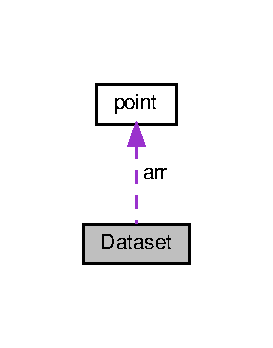
\includegraphics[width=131pt]{classDataset__coll__graph}
\end{center}
\end{figure}
\subsection*{Public Member Functions}
\begin{DoxyCompactItemize}
\item 
\hyperlink{classDataset_a2ef0a4a688a218d55ef061c6df659a4a}{Dataset} ()
\item 
void \hyperlink{classDataset_ad5ab44474be3c0648df25f3752916576}{new\+\_\+point} (float x, float y)
\end{DoxyCompactItemize}
\subsection*{Public Attributes}
\begin{DoxyCompactItemize}
\item 
int \hyperlink{classDataset_aed9a6877e5e1483ea47d1f6e39e404f0}{index} =0
\item 
\hyperlink{classpoint}{point} $\ast$$\ast$ \hyperlink{classDataset_acd70fa206d8b0a819a07a658f700f9bf}{arr}
\end{DoxyCompactItemize}


\subsection{Detailed Description}
A class for the dataset  A constructor to initialize with number of points and an array to store points. 

\subsection{Constructor \& Destructor Documentation}
\mbox{\Hypertarget{classDataset_a2ef0a4a688a218d55ef061c6df659a4a}\label{classDataset_a2ef0a4a688a218d55ef061c6df659a4a}} 
\index{Dataset@{Dataset}!Dataset@{Dataset}}
\index{Dataset@{Dataset}!Dataset@{Dataset}}
\subsubsection{\texorpdfstring{Dataset()}{Dataset()}}
{\footnotesize\ttfamily Dataset\+::\+Dataset (\begin{DoxyParamCaption}{ }\end{DoxyParamCaption})\hspace{0.3cm}{\ttfamily [inline]}}

Defines an array of required size

\subsection{Member Function Documentation}
\mbox{\Hypertarget{classDataset_ad5ab44474be3c0648df25f3752916576}\label{classDataset_ad5ab44474be3c0648df25f3752916576}} 
\index{Dataset@{Dataset}!new\+\_\+point@{new\+\_\+point}}
\index{new\+\_\+point@{new\+\_\+point}!Dataset@{Dataset}}
\subsubsection{\texorpdfstring{new\+\_\+point()}{new\_point()}}
{\footnotesize\ttfamily void Dataset\+::new\+\_\+point (\begin{DoxyParamCaption}\item[{float}]{x,  }\item[{float}]{y }\end{DoxyParamCaption})\hspace{0.3cm}{\ttfamily [inline]}}

Adds a point to the datasetHere is the caller graph for this function\+:\nopagebreak
\begin{figure}[H]
\begin{center}
\leavevmode
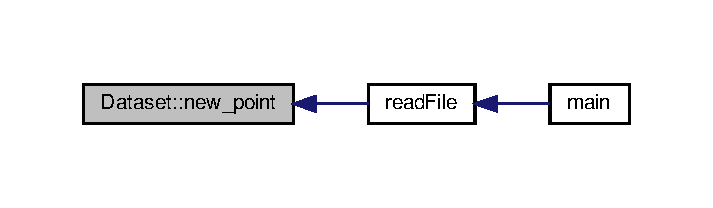
\includegraphics[width=342pt]{classDataset_ad5ab44474be3c0648df25f3752916576_icgraph}
\end{center}
\end{figure}


\subsection{Member Data Documentation}
\mbox{\Hypertarget{classDataset_acd70fa206d8b0a819a07a658f700f9bf}\label{classDataset_acd70fa206d8b0a819a07a658f700f9bf}} 
\index{Dataset@{Dataset}!arr@{arr}}
\index{arr@{arr}!Dataset@{Dataset}}
\subsubsection{\texorpdfstring{arr}{arr}}
{\footnotesize\ttfamily \hyperlink{classpoint}{point}$\ast$$\ast$ Dataset\+::arr}

\mbox{\Hypertarget{classDataset_aed9a6877e5e1483ea47d1f6e39e404f0}\label{classDataset_aed9a6877e5e1483ea47d1f6e39e404f0}} 
\index{Dataset@{Dataset}!index@{index}}
\index{index@{index}!Dataset@{Dataset}}
\subsubsection{\texorpdfstring{index}{index}}
{\footnotesize\ttfamily int Dataset\+::index =0}



The documentation for this class was generated from the following file\+:\begin{DoxyCompactItemize}
\item 
\hyperlink{bestfit_8cpp}{bestfit.\+cpp}\end{DoxyCompactItemize}

\hypertarget{classerrorxy}{}\section{errorxy Class Reference}
\label{classerrorxy}\index{errorxy@{errorxy}}


A class for error  The slope,intercept and error values.  


\subsection*{Public Attributes}
\begin{DoxyCompactItemize}
\item 
float \hyperlink{classerrorxy_a78038a0cf07f5680a7b48a0bfb6883d3}{slope}
\item 
float \hyperlink{classerrorxy_a0f40aaf1eace64d0e7c99446bf5ef33c}{intercept}
\item 
float \hyperlink{classerrorxy_a490a191956280cecef74afb23e134073}{e}
\end{DoxyCompactItemize}


\subsection{Detailed Description}
A class for error  The slope,intercept and error values. 

\subsection{Member Data Documentation}
\mbox{\Hypertarget{classerrorxy_a490a191956280cecef74afb23e134073}\label{classerrorxy_a490a191956280cecef74afb23e134073}} 
\index{errorxy@{errorxy}!e@{e}}
\index{e@{e}!errorxy@{errorxy}}
\subsubsection{\texorpdfstring{e}{e}}
{\footnotesize\ttfamily float errorxy\+::e}

\mbox{\Hypertarget{classerrorxy_a0f40aaf1eace64d0e7c99446bf5ef33c}\label{classerrorxy_a0f40aaf1eace64d0e7c99446bf5ef33c}} 
\index{errorxy@{errorxy}!intercept@{intercept}}
\index{intercept@{intercept}!errorxy@{errorxy}}
\subsubsection{\texorpdfstring{intercept}{intercept}}
{\footnotesize\ttfamily float errorxy\+::intercept}

\mbox{\Hypertarget{classerrorxy_a78038a0cf07f5680a7b48a0bfb6883d3}\label{classerrorxy_a78038a0cf07f5680a7b48a0bfb6883d3}} 
\index{errorxy@{errorxy}!slope@{slope}}
\index{slope@{slope}!errorxy@{errorxy}}
\subsubsection{\texorpdfstring{slope}{slope}}
{\footnotesize\ttfamily float errorxy\+::slope}



The documentation for this class was generated from the following file\+:\begin{DoxyCompactItemize}
\item 
\hyperlink{bestfit_8cpp}{bestfit.\+cpp}\end{DoxyCompactItemize}

\hypertarget{classpoint}{}\section{point Class Reference}
\label{classpoint}\index{point@{point}}


A class for point  The coordinates and a constructor.  


\subsection*{Public Member Functions}
\begin{DoxyCompactItemize}
\item 
\hyperlink{classpoint_a126b72c139d88abce764b54c967acfb8}{point} (float a, float b)
\end{DoxyCompactItemize}
\subsection*{Public Attributes}
\begin{DoxyCompactItemize}
\item 
float \hyperlink{classpoint_a8293fd2de3ce739deb6d53691fd21fcf}{x}
\item 
float \hyperlink{classpoint_a616ad85a2096d1566f5971666bbc3b3f}{y}
\end{DoxyCompactItemize}


\subsection{Detailed Description}
A class for point  The coordinates and a constructor. 

\subsection{Constructor \& Destructor Documentation}
\mbox{\Hypertarget{classpoint_a126b72c139d88abce764b54c967acfb8}\label{classpoint_a126b72c139d88abce764b54c967acfb8}} 
\index{point@{point}!point@{point}}
\index{point@{point}!point@{point}}
\subsubsection{\texorpdfstring{point()}{point()}}
{\footnotesize\ttfamily point\+::point (\begin{DoxyParamCaption}\item[{float}]{a,  }\item[{float}]{b }\end{DoxyParamCaption})\hspace{0.3cm}{\ttfamily [inline]}}

Intialize the values for point

\subsection{Member Data Documentation}
\mbox{\Hypertarget{classpoint_a8293fd2de3ce739deb6d53691fd21fcf}\label{classpoint_a8293fd2de3ce739deb6d53691fd21fcf}} 
\index{point@{point}!x@{x}}
\index{x@{x}!point@{point}}
\subsubsection{\texorpdfstring{x}{x}}
{\footnotesize\ttfamily float point\+::x}

\mbox{\Hypertarget{classpoint_a616ad85a2096d1566f5971666bbc3b3f}\label{classpoint_a616ad85a2096d1566f5971666bbc3b3f}} 
\index{point@{point}!y@{y}}
\index{y@{y}!point@{point}}
\subsubsection{\texorpdfstring{y}{y}}
{\footnotesize\ttfamily float point\+::y}



The documentation for this class was generated from the following file\+:\begin{DoxyCompactItemize}
\item 
\hyperlink{bestfit_8cpp}{bestfit.\+cpp}\end{DoxyCompactItemize}

\chapter{File Documentation}
\hypertarget{bestfit_8cpp}{}\section{bestfit.\+cpp File Reference}
\label{bestfit_8cpp}\index{bestfit.\+cpp@{bestfit.\+cpp}}


Basic functionality.  This file has all the classes and functions needed to find the bestfit line. It is called by the Python script everytime the slider is changed.  


{\ttfamily \#include $<$bits/stdc++.\+h$>$}\newline
{\ttfamily \#include $<$iostream$>$}\newline
{\ttfamily \#include $<$string$>$}\newline
Include dependency graph for bestfit.\+cpp\+:\nopagebreak
\begin{figure}[H]
\begin{center}
\leavevmode
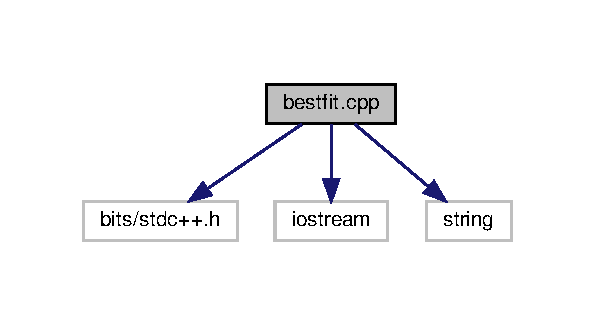
\includegraphics[width=286pt]{bestfit_8cpp__incl}
\end{center}
\end{figure}
\subsection*{Classes}
\begin{DoxyCompactItemize}
\item 
class \hyperlink{classpoint}{point}
\begin{DoxyCompactList}\small\item\em A class for point  The coordinates and a constructor. \end{DoxyCompactList}\item 
class \hyperlink{classerrorxy}{errorxy}
\begin{DoxyCompactList}\small\item\em A class for error  The slope,intercept and error values. \end{DoxyCompactList}\item 
class \hyperlink{classDataset}{Dataset}
\begin{DoxyCompactList}\small\item\em A class for the dataset  A constructor to initialize with number of points and an array to store points. \end{DoxyCompactList}\end{DoxyCompactItemize}
\subsection*{Functions}
\begin{DoxyCompactItemize}
\item 
void \hyperlink{bestfit_8cpp_a27428b63bcf403c94d1f4500552b9ddd}{err} (\hyperlink{classDataset}{Dataset} $\ast$temp)
\item 
void \hyperlink{bestfit_8cpp_a9be2a8d43d108e4fdc81aab7b731ec0c}{read\+File} (\hyperlink{classDataset}{Dataset} $\ast$D)
\item 
int \hyperlink{bestfit_8cpp_a3c04138a5bfe5d72780bb7e82a18e627}{main} (int argc, char $\ast$$\ast$argv)
\end{DoxyCompactItemize}
\subsection*{Variables}
\begin{DoxyCompactItemize}
\item 
int \hyperlink{bestfit_8cpp_abaef4f818f7fb7047b746a6cdd2bfdda}{num\+\_\+points}
\begin{DoxyCompactList}\small\item\em A G\+L\+O\+B\+AL V\+A\+R\+I\+A\+B\+LE H\+O\+L\+D\+I\+NG T\+HE N\+U\+M\+B\+ER OF P\+O\+I\+N\+TS. \end{DoxyCompactList}\item 
int \hyperlink{bestfit_8cpp_a3d4657665bf2dafc64e4960fd22279c8}{D\+\_\+size}
\begin{DoxyCompactList}\small\item\em A G\+L\+O\+B\+AL V\+A\+R\+I\+A\+B\+LE TO S\+T\+O\+RE T\+HE S\+I\+ZE OF D\+A\+T\+A\+S\+ET. \end{DoxyCompactList}\item 
float \hyperlink{bestfit_8cpp_ae78103ab33f03590e84ff7bc735629d7}{c}
\begin{DoxyCompactList}\small\item\em A G\+L\+O\+B\+AL V\+A\+R\+I\+A\+B\+LE F\+OR V\+A\+L\+UE OF P\+E\+N\+A\+L\+TY C. \end{DoxyCompactList}\item 
float $\ast$ \hyperlink{bestfit_8cpp_a4eb4b863ad1d4745ea0bfbeebfa26326}{OP}
\begin{DoxyCompactList}\small\item\em A G\+L\+O\+B\+AL P\+O\+I\+N\+T\+ER TO S\+T\+O\+RE T\+HE 1-\/D A\+R\+R\+AY F\+OR DP. \end{DoxyCompactList}\item 
int $\ast$ \hyperlink{bestfit_8cpp_a7a923560494f659a6ebc84bb50f47e50}{minarr}
\begin{DoxyCompactList}\small\item\em A P\+O\+I\+N\+T\+ER TO S\+T\+O\+RE T\+HE A\+R\+R\+AY F\+OR T\+HE P\+A\+TH R\+E\+C\+O\+N\+S\+T\+R\+U\+C\+T\+I\+ON. \end{DoxyCompactList}\item 
\hyperlink{classerrorxy}{errorxy} $\ast$$\ast$ \hyperlink{bestfit_8cpp_a85ac310846072bf4d0bede011558acf1}{perr}
\begin{DoxyCompactList}\small\item\em A G\+L\+O\+B\+AL P\+O\+I\+N\+T\+ER TO P\+O\+I\+N\+T\+E\+RS TO F\+O\+RM T\+HE 2-\/D A\+R\+R\+AY. \end{DoxyCompactList}\end{DoxyCompactItemize}


\subsection{Detailed Description}
Basic functionality.  This file has all the classes and functions needed to find the bestfit line. It is called by the Python script everytime the slider is changed. 

\begin{DoxyAuthor}{Author}
Ansuman 
\end{DoxyAuthor}


\subsection{Function Documentation}
\mbox{\Hypertarget{bestfit_8cpp_a27428b63bcf403c94d1f4500552b9ddd}\label{bestfit_8cpp_a27428b63bcf403c94d1f4500552b9ddd}} 
\index{bestfit.\+cpp@{bestfit.\+cpp}!err@{err}}
\index{err@{err}!bestfit.\+cpp@{bestfit.\+cpp}}
\subsubsection{\texorpdfstring{err()}{err()}}
{\footnotesize\ttfamily void err (\begin{DoxyParamCaption}\item[{\hyperlink{classDataset}{Dataset} $\ast$}]{temp }\end{DoxyParamCaption})}

Utility function for finding out the error of best fit line between any two points , Output = A 2d matrix with error valuesHere is the caller graph for this function\+:\nopagebreak
\begin{figure}[H]
\begin{center}
\leavevmode
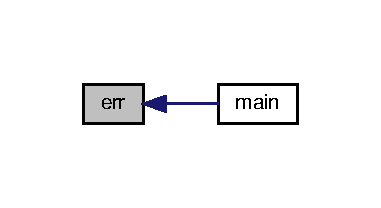
\includegraphics[width=183pt]{bestfit_8cpp_a27428b63bcf403c94d1f4500552b9ddd_icgraph}
\end{center}
\end{figure}
\mbox{\Hypertarget{bestfit_8cpp_a3c04138a5bfe5d72780bb7e82a18e627}\label{bestfit_8cpp_a3c04138a5bfe5d72780bb7e82a18e627}} 
\index{bestfit.\+cpp@{bestfit.\+cpp}!main@{main}}
\index{main@{main}!bestfit.\+cpp@{bestfit.\+cpp}}
\subsubsection{\texorpdfstring{main()}{main()}}
{\footnotesize\ttfamily int main (\begin{DoxyParamCaption}\item[{int}]{argc,  }\item[{char $\ast$$\ast$}]{argv }\end{DoxyParamCaption})}

Here is the call graph for this function\+:\nopagebreak
\begin{figure}[H]
\begin{center}
\leavevmode
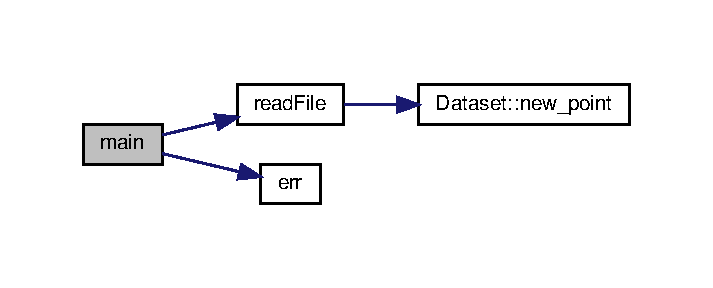
\includegraphics[width=342pt]{bestfit_8cpp_a3c04138a5bfe5d72780bb7e82a18e627_cgraph}
\end{center}
\end{figure}
\mbox{\Hypertarget{bestfit_8cpp_a9be2a8d43d108e4fdc81aab7b731ec0c}\label{bestfit_8cpp_a9be2a8d43d108e4fdc81aab7b731ec0c}} 
\index{bestfit.\+cpp@{bestfit.\+cpp}!read\+File@{read\+File}}
\index{read\+File@{read\+File}!bestfit.\+cpp@{bestfit.\+cpp}}
\subsubsection{\texorpdfstring{read\+File()}{readFile()}}
{\footnotesize\ttfamily void read\+File (\begin{DoxyParamCaption}\item[{\hyperlink{classDataset}{Dataset} $\ast$}]{D }\end{DoxyParamCaption})}

Utility function to read the file and add points to the \hyperlink{classDataset}{Dataset}Here is the call graph for this function\+:\nopagebreak
\begin{figure}[H]
\begin{center}
\leavevmode
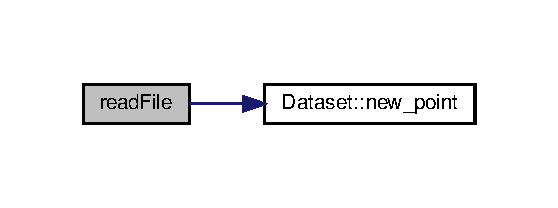
\includegraphics[width=268pt]{bestfit_8cpp_a9be2a8d43d108e4fdc81aab7b731ec0c_cgraph}
\end{center}
\end{figure}
Here is the caller graph for this function\+:\nopagebreak
\begin{figure}[H]
\begin{center}
\leavevmode
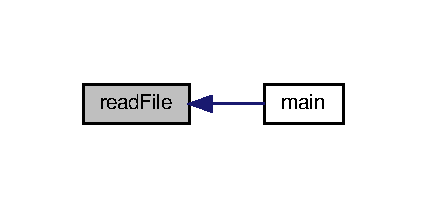
\includegraphics[width=205pt]{bestfit_8cpp_a9be2a8d43d108e4fdc81aab7b731ec0c_icgraph}
\end{center}
\end{figure}


\subsection{Variable Documentation}
\mbox{\Hypertarget{bestfit_8cpp_ae78103ab33f03590e84ff7bc735629d7}\label{bestfit_8cpp_ae78103ab33f03590e84ff7bc735629d7}} 
\index{bestfit.\+cpp@{bestfit.\+cpp}!c@{c}}
\index{c@{c}!bestfit.\+cpp@{bestfit.\+cpp}}
\subsubsection{\texorpdfstring{c}{c}}
{\footnotesize\ttfamily float c}



A G\+L\+O\+B\+AL V\+A\+R\+I\+A\+B\+LE F\+OR V\+A\+L\+UE OF P\+E\+N\+A\+L\+TY C. 

\mbox{\Hypertarget{bestfit_8cpp_a3d4657665bf2dafc64e4960fd22279c8}\label{bestfit_8cpp_a3d4657665bf2dafc64e4960fd22279c8}} 
\index{bestfit.\+cpp@{bestfit.\+cpp}!D\+\_\+size@{D\+\_\+size}}
\index{D\+\_\+size@{D\+\_\+size}!bestfit.\+cpp@{bestfit.\+cpp}}
\subsubsection{\texorpdfstring{D\+\_\+size}{D\_size}}
{\footnotesize\ttfamily int D\+\_\+size}



A G\+L\+O\+B\+AL V\+A\+R\+I\+A\+B\+LE TO S\+T\+O\+RE T\+HE S\+I\+ZE OF D\+A\+T\+A\+S\+ET. 

\mbox{\Hypertarget{bestfit_8cpp_a7a923560494f659a6ebc84bb50f47e50}\label{bestfit_8cpp_a7a923560494f659a6ebc84bb50f47e50}} 
\index{bestfit.\+cpp@{bestfit.\+cpp}!minarr@{minarr}}
\index{minarr@{minarr}!bestfit.\+cpp@{bestfit.\+cpp}}
\subsubsection{\texorpdfstring{minarr}{minarr}}
{\footnotesize\ttfamily int$\ast$ minarr}



A P\+O\+I\+N\+T\+ER TO S\+T\+O\+RE T\+HE A\+R\+R\+AY F\+OR T\+HE P\+A\+TH R\+E\+C\+O\+N\+S\+T\+R\+U\+C\+T\+I\+ON. 

\mbox{\Hypertarget{bestfit_8cpp_abaef4f818f7fb7047b746a6cdd2bfdda}\label{bestfit_8cpp_abaef4f818f7fb7047b746a6cdd2bfdda}} 
\index{bestfit.\+cpp@{bestfit.\+cpp}!num\+\_\+points@{num\+\_\+points}}
\index{num\+\_\+points@{num\+\_\+points}!bestfit.\+cpp@{bestfit.\+cpp}}
\subsubsection{\texorpdfstring{num\+\_\+points}{num\_points}}
{\footnotesize\ttfamily int num\+\_\+points}



A G\+L\+O\+B\+AL V\+A\+R\+I\+A\+B\+LE H\+O\+L\+D\+I\+NG T\+HE N\+U\+M\+B\+ER OF P\+O\+I\+N\+TS. 

\mbox{\Hypertarget{bestfit_8cpp_a4eb4b863ad1d4745ea0bfbeebfa26326}\label{bestfit_8cpp_a4eb4b863ad1d4745ea0bfbeebfa26326}} 
\index{bestfit.\+cpp@{bestfit.\+cpp}!OP@{OP}}
\index{OP@{OP}!bestfit.\+cpp@{bestfit.\+cpp}}
\subsubsection{\texorpdfstring{OP}{OP}}
{\footnotesize\ttfamily float$\ast$ OP}



A G\+L\+O\+B\+AL P\+O\+I\+N\+T\+ER TO S\+T\+O\+RE T\+HE 1-\/D A\+R\+R\+AY F\+OR DP. 

\mbox{\Hypertarget{bestfit_8cpp_a85ac310846072bf4d0bede011558acf1}\label{bestfit_8cpp_a85ac310846072bf4d0bede011558acf1}} 
\index{bestfit.\+cpp@{bestfit.\+cpp}!perr@{perr}}
\index{perr@{perr}!bestfit.\+cpp@{bestfit.\+cpp}}
\subsubsection{\texorpdfstring{perr}{perr}}
{\footnotesize\ttfamily \hyperlink{classerrorxy}{errorxy}$\ast$$\ast$ perr}



A G\+L\+O\+B\+AL P\+O\+I\+N\+T\+ER TO P\+O\+I\+N\+T\+E\+RS TO F\+O\+RM T\+HE 2-\/D A\+R\+R\+AY. 


\hypertarget{vis_8py}{}\section{vis.\+py File Reference}
\label{vis_8py}\index{vis.\+py@{vis.\+py}}
\subsection*{Namespaces}
\begin{DoxyCompactItemize}
\item 
 \hyperlink{namespacevis}{vis}
\end{DoxyCompactItemize}
\subsection*{Functions}
\begin{DoxyCompactItemize}
\item 
def \hyperlink{namespacevis_a987b76332d0d03b66af97331e5e4b442}{vis.\+get\+Val} (event)
\end{DoxyCompactItemize}
\subsection*{Variables}
\begin{DoxyCompactItemize}
\item 
int \hyperlink{namespacevis_a670f391917319e53a1373004ad47a325}{vis.\+n\+\_\+points} = 10
\item 
\hyperlink{namespacevis_a4086117aa0dbd872a99b2f3738d56ae6}{vis.\+x\+\_\+pure} = np.\+linspace(-\/n\+\_\+points,n\+\_\+points,n\+\_\+points)
\item 
\hyperlink{namespacevis_ac14aca4ab4de023eb6759df589da3396}{vis.\+y\+\_\+pure} = x\+\_\+pure
\item 
list \hyperlink{namespacevis_ac930396acd65d715184cfd4ae2df301c}{vis.\+noise\+\_\+points} = \mbox{[}i\mbox{[}0\mbox{]} for i in (n\+\_\+points$\ast$np.\+random.\+rand(n\+\_\+points,1) -\/ n\+\_\+points/2)\mbox{]}
\item 
\hyperlink{namespacevis_a6ee13a8bd702057064f342e00fe8eefd}{vis.\+master} = Tk()
\item 
\hyperlink{namespacevis_a294e676e5dc073fa5ddcea9955943af9}{vis.\+Throttle} = Scale(master, from\+\_\+=0, to=100$\ast$n\+\_\+points,resolution=0.\+1, orient=H\+O\+R\+I\+Z\+O\+N\+T\+AL, width=40, length=1000, command=get\+Val)
\end{DoxyCompactItemize}

%--- End generated contents ---

% Index
\backmatter
\newpage
\phantomsection
\clearemptydoublepage
\addcontentsline{toc}{chapter}{Index}
\printindex

\end{document}
